\documentclass{superfri}
\usepackage[T2A]{fontenc}
\usepackage[utf8]{inputenc}
\usepackage{amsmath}
\usepackage{amssymb}
\usepackage{amsthm}
\usepackage{mathrsfs}
\usepackage{booktabs}
\usepackage{multirow}
\usepackage{makecell}
\usepackage{float}
\usepackage{algorithm}
\usepackage{algpseudocode}
\usepackage[normalem]{ulem}
\usepackage{graphicx}
\usepackage{lmodern}
\usepackage[hidelinks]{hyperref}

\begin{document}
\raggedbottom
\author{D.\,A.~Grigoriev\footnote{\label{msu}Lomonosov Moscow State University, Moscow Center for Fundamental and Applied Mathematics, \\ Moscow, Russian Federation}\footnote{E-mail: dagrig14@yandex.ru} \and D.\,V.~Khudiakov\footnoteref{msu}\footnote{E-mail: hydikovv17914@gmail.com} \and D.\,I.~Chernyshev\footnoteref{msu}\footnote{E-mail: chdanorbis@yandex.ru}}

\title{Literature summarization with large language models}

\maketitle{}

\begin{abstract}
The work is dedicated to automatic summarization of Russian literary fiction.
An open corpus RuBookSum (600+ "book-summary" pairs) was compiled based on texts from LibRuSec and user-generated summaries from <<Народный Брифли>>.
Four approaches to summarization are examined: the baseline hierarchical method and the "blueprint" (Text-Blueprint) approach, 
which builds an outline in the form of question-answer pairs, as well as two new methods proposed in this work: 
a hierarchical method with node filtering based on cosine similarity of embeddings, 
and a modification of the blueprint approach with question clustering using the KMeans algorithm.
The best quality is achieved by Qwen3-235B-A22B in the blueprint method, 
while the hierarchical method with filtering provides the best balance between generation time and quality.
\keywords{LLM, summarization, literature, books, brief retelling}
\end{abstract}



% ================= ВВЕДЕНИЕ =================
\section*{Introduction}
Automatic text summarization is one of the key tasks in natural language processing. The goal is to create an informative summary of the source text while preserving its main meaning.
In recent years, with the advent of large language models (LLMs), interest in automating summarization has increased across many genres, including fiction.
Unlike scientific, news, or technical texts, fiction is characterized by high stylistic and semantic complexity.
Non-linear storytelling, imagery, metaphor, and stylistic devices make short synopsis writing especially challenging.
The limited context window of modern models further complicates processing long works.

At present moment there are not many datasets focusing specifically on summarizing fiction, and the key open datasets concentrate on non-Russian material.
BookSum \cite{BookSum} is one of the first and best-known English-language datasets for abstractive summarization of narrative works. 
It contains books, plays, and short stories paired with summaries of varying granularity (paragraph level, chapter level, book level).
Echoes from Alexandria \cite{alexandria} is a multilingual corpus of fiction, including five languages: English, German, French, Italian, and Spanish.
FABLES \cite{fables} is a hand-curated corpus designed to evaluate factual faithfulness of summaries for book-length fiction.
It includes 3,158 claims extracted from LLM-generated summaries for 26 books.
Each claim is evaluated across model outputs by experts.
According to FABLES, even advanced models (e.g., Claude) commit 20–30\% factual errors, including distorted
causal relations, incorrect characterization of protagonists, and overemphasis on minor details,
judged by three criteria: agreement with original events, logical correctness, and absence of distortions.

In theory, automatic summarization can be performed in two main ways: extractive (selecting key text fragments) and abstractive (generating new text based on the source).
For prose, abstractive summarization is typically chosen:
key meanings and plot links are distributed throughout the text, so extractive sentence selection yields a fragmented,
stylistically uneven result and does not reconstruct the plot, therefore abstractive approach was chosen.

The topic is motivated by the growing need for tools capable of automatically producing concise, informative, and stylistically appropriate synopses for works of fiction.
The goal of this work is to provide such tools, thus, following is proposed:
\begin{enumerate}
  \item New Russian-language dataset that includes literary works and their synopses;
  \item New summarization methods that offer alternatives to existing ones and substantially reduce the time required to produce a short synopsis of a book.
\end{enumerate}

Code and data are publicly available\footnote{\label{git}\url{https://github.com/Nejimaki-Tori/BookSum}}.

% ================= НАБОР ДАННЫХ =================

\section{Dataset}
At the start of the study, there were no open and representative corpora designed specifically for summarizing fiction in Russian.
To run experiments and evaluate different approaches, we created our own corpus consisting of works of fiction and corresponding short synopses.
As the source of synopses we used the "Narodny Briefly" platform \cite{Briefly} where users publish short summaries of literary works.

The synopses are user-generated texts based on the original works. They vary in length-from a few sentences to several paragraphs-and in style: some reproduce key phrases verbatim, 
while others use freer narration. Some cover the whole work, others split content by chapter.
Usually they contain the main facts and conclusions from the source text, but may include the author’s commentary.

The book texts were selected from the LibRuSec electronic library \cite{librusec}, one of the largest Russian-language fiction resources.
Works were selected for which a synopsis existed on chosen source\cite{Briefly}. Each text underwent automatic preprocessing: meta-information (e.g., titles, chapter descriptions, technical inserts) was removed,
then the text was formatted into a unified, standardized form suitable for use with models.

To better link books with their synopses, semantic similarity was used: the author name text from Briefly \cite{Briefly} and from LibRuSec \cite{librusec} was embedded via SentenceTransformer
with the model\footnote{\label{encoder}\url{https://huggingface.co/deepvk/USER-bge-m3}}
and compared using cosine similarity.

\tab{tab:dataset_info}{Dataset overview}{
\begin{tabular}{l|cccc}
\hline
\textbf{Dataset} & \makecell{Number of \\ documents} & \makecell{Avg. document \\ length \\ (\# words)} & \makecell{Avg. summary \\ length \\ (\# words)} & \makecell{Compression ratio \\ (summary length \\/ text length)} \\
\hline
\textbf{RuBookSum}  & 634 & 35052.64 & 700.77 & 8.43\% \\
\hline
BookSum    & 405 & 112885.15 & 1167.20 & 0.79\% \\
Gazeta     & 60964 & 632.77 & 41.94 & 6.99\% \\
\hline
\end{tabular}
}

The synopses were automatically cleaned of HTML tags, comments, and service markers using LLM Meta-\allowbreak Llama 3-\allowbreak 70B-\allowbreak Instruct.
Then LibRuSec was searched and a collection of "book text – synopsis" pairs was formed.
\\The resulting corpus includes:
\begin{itemize}
  \item 600+ cleaned user synopses from "Narodny Briefly" \cite{Briefly};
  \item 40+ different genres;
  \item source works from the LibRuSec electronic library \cite{librusec}.
\end{itemize}
\begin{figure}[!htbp]
    \centering
    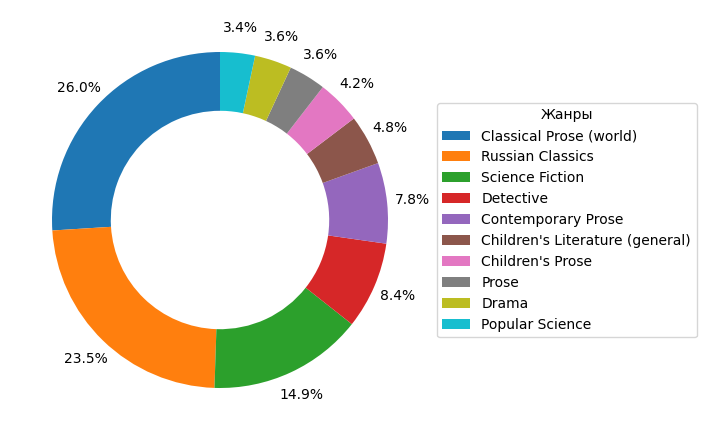
\includegraphics[width=0.8\linewidth]{figures/genres_pie.png}
    \caption{Distribution of texts by genres (top 10 genres)}
    \label{fig:genres}
\end{figure}
Figure \ref{fig:genres} shows the genre distribution in the collection. Table \tabref{tab:dataset_info} gives dataset statistics versus analogs.

% ================= МЕТОДОЛОГИЯ =================
\section{Methodology}
\subsection{Baseline and modified strategies.}

\subsubsection{Hierarchical method (Algorithm 1).}
This method \cite{hierarchical} splits the text into fragments (chunks) and
generates a local summary for each chunk.
These fragments are then grouped, and summaries are merged into higher-level synopses.
The last level yields the final book-level summary.

\subsubsection{Hierarchical method with node filtering (Algorithm 2).}
The classical hierarchical method constructs the final summary through a multi-layered combination of intermediate obtained derived from individual text segments.
However, literary works often contain segments that have little impact on plot development and include numerous redundant repetitions and minor details. 
During the generation of the final summary, these segments can reduce its informativeness and, in some cases, even interfere with the model at the stage of summarizing individual fragments.

To address this issue, a node filtering mechanism based on semantic similarity was implemented into the method.
To eliminate low-informative or redundant fragments, a global check of semantic similarity between all intermediate summaries is performed at each hierarchy level.
Fragments that are close in cosine similarity to previous ones are considered redundant and are not used for compiling the summary at the current level.
Embeddings are obtained using SentenceTransformer (the USER-bge-m3 model), and processing is performed at high speed on a GPU.
This modification aims to accelerate generation by removing potentially superfluous parts of information, thereby increasing the density of useful information in the final summaries.

\noindent
\begin{minipage}[t]{0.49\textwidth}
  \begin{algorithm}[H]
  \caption{Hierarchical method}
    \begin{algorithmic}
      \Require $W$ - model context window, $D$ - input text of length $L \gg W$, $p_\theta$ - model, $C$ - chunk length
      \State Split $D$ into chunks $c_1\dots c_{\lceil \frac{L}{C} \rceil}$
      \For{$c_i=c_1\dots c_{\lceil \frac{L}{C} \rceil}$}
        \State $S_0 \gets SummarizeChunk(p_\theta, c_i)$\
      \EndFor
      \Repeat
        \State $Groups \gets GroupSummaries(S_l)$
        \State $\ell \gets \ell + 1$
        \For{$g \in Groups$}
          \State $S_l \gets \{MergeGroup(p_\theta,g)\}$
        \EndFor
      \Until{$|S_l|=1$}
      \State \Return $S_l[1]$
    \end{algorithmic}
  \end{algorithm}
\end{minipage}\hfill
\begin{minipage}[t]{0.49\textwidth}
  \begin{algorithm}[H]
    \caption{Hierarchical method with filtering}
    \begin{algorithmic}
      \Require $W$ - model context window, $D$ - input text of length $L \gg W$, $p_\theta$ - model, $\theta$ - similarity threshold, $C$ - chunk length
      \State Split $D$ into chunks $c_1\dots c_{\lceil \frac{L}{C} \rceil}$
      \State $S_0 \gets \{c_1\dots c_{\lceil \frac{L}{C} \rceil}\}$
      \Repeat
        \For{$s_i \in S_l$}
          \State $e_i \gets Encoder(s_i)$
          \State $M_{ij} \gets \dfrac{\mathbf{e}_i\cdot \mathbf{e}_j}{\|\mathbf{e}_i\|\,\|\mathbf{e}_j\|}$\Comment{Embedding matrix}
          \State Compute the maximum similarity
        \State with previous summaries.
          \State $m_j=\max_{i<j} M_{ji}$
          \State $S_l \gets \{s_i \mid m_i < \theta$ \textbf{ or } $i = 0 \}$ \Comment{Filtering}
        \EndFor
        \State $Groups \gets GroupSummaries(S_l)$
        \State $\ell \gets \ell + 1$
        \For{$g \in Groups$}
          \State $S_l \gets \{MergeGroup(p_\theta,g)\}$
        \EndFor
      \Until{$|S_l|=1$}
      \State \Return $S_l[1]$
    \end{algorithmic}
  \end{algorithm}
\end{minipage}

\vspace{0.4em}
\subsubsection{Text-Blueprint (Algorithm 3).}
This method \cite{blueprint} is essentially a modification of the hierarchical approach and focuses on building an intermediate plan before text generation.
The outline is formed as a set of question-answer pairs, which enhances the controllability of the generation process and ensures the structured nature of the result.
First the model creates a list of questions reflecting key events, themes, and characters. Then short answers are automatically generated for each question.
This structure serves as a blueprint used to produce the final synopsis.


\subsubsection{Blueprint method with question clustering (Algorithm 4).}
The baseline blueprint implementation generates a question-answer plan for each fragment and at each aggregation level. 
With fiction, however, questions produced for different chunks may overlap and yield conflicting answers, which in turn confuses aggregation, making the synopsis less structured and complete. 
Moreover, generating a plan at every step slows the method and consumes extra LLM time.
To reduce model calls and improve structure, we added clustering of questions using SentenceTransformers and K-means.

\noindent
\begin{minipage}[t]{0.49\textwidth}
  \begin{algorithm}[H]
    \caption{Blueprint method}
    \begin{algorithmic}
      \Require $W$ - model context window, $D$ - input text of length $L \gg W$, $p_\theta$ - model, $C$ - chunk length, $R$ - length limit
      \State Split $D$ into chunks $c_1\dots c_{\lceil \frac{L}{C} \rceil}$
      \For{$c_i=c_1\dots c_{\lceil \frac{L}{C} \rceil}$}
        \State $b_i \gets GenerateBlueprint(p_\theta, c_i)$\
        \State $S_0 \gets \{SumWithBp(p_\theta, b_i, c_i)\}$\
      \EndFor
      \Repeat \Comment{Merging summaries}
        \State $Groups \gets GroupSummaries(S_l)$
        \State $\ell \gets \ell + 1$
        \For{$g \in Groups$}
          \If{$Length(g) > R$}
            \State $b_i \gets GenerateBlueprint(p_\theta, g)$\
            \State $S_l \gets \{SumWithBp(p_\theta, b_i, g)\}$\
          \Else
            \State $S_l \gets \{g\}$\
          \EndIf
        \EndFor
      \Until{$|S_l|=1$}
      \State \Return $S_l[1]$
    \end{algorithmic}
  \end{algorithm}
\end{minipage}\hfill
\begin{minipage}[t]{0.49\textwidth}
  \begin{algorithm}[H]
  \caption{Blueprint method with clustering}
      \begin{algorithmic}
        \Require $W$ - model context window, $D$ - input text of length $L \gg W$, $p_\theta$ - model, $C$ - chunk length, $R$ - length limit
        \State Split $D$ into chunks $c_1\dots c_{\lceil \frac{L}{C} \rceil}$
        \For{$c_i=c_1\dots c_{\lceil \frac{L}{C} \rceil}$}
          \State $b_i \gets GenerateBlueprint(p_\theta, c_i)$
          \State $Q \gets \{ExtractQuestions(p_\theta, b_i)\}$
        \EndFor
        \For{$q_i \in Q$}
          \State $E \gets \{Encoder(q_i)\}$
          \State $K \gets KMeans(E)$
          \For{$k_i \in K$}
            \State $q_i \gets Generalize(p_\theta, k_i)$
            \State $Q \gets \{q_i\}$ \Comment{Build a global plan}
          \EndFor
          \For{$c_i=c_1\dots c_{\lceil \frac{L}{C} \rceil}$}
            \State $S_0 \gets \{SumWithBp(p_\theta, b_i, c_i)\}$\
          \EndFor
        \EndFor
        \State \textbf{Merge summaries} as in the Blueprint method, except the blueprint here is the single global plan $Q$.
      \end{algorithmic}
  \end{algorithm}
\end{minipage}

% ================= МЕТРИКИ =================

\section{Metrics}

For an objective comparison of the described approaches and models in the task of summarizing literary texts, four groups of metrics were used.

\textbf{ROUGE-L} \cite{rouge} - based on the length of the longest common subsequence (LCS) between the generated summary $S$ and the reference $R$.
\begin{equation}
  \text{Precision} = \frac{\mathrm{LCS}(S,R)}{|S|},\quad
\end{equation}
\begin{equation}
  \text{Recall} = \frac{\mathrm{LCS}(S,R)}{|R|}
\end{equation}
\begin{equation}
  \text{ROUGE-L} = \frac{2\;\text{Precision}\;\cdot\;\text{Recall}}{\text{Precision} + \text{Recall}}
\end{equation}

\textbf{BERTScore} \cite{bertscore} - semantic quality at token level. For every token pair from prediction and reference we compute cosine similarity of their embeddings in USER-bge-m3. Then:
\begin{equation}
P = \frac{1}{|S|}\sum_{t\in S}\max_{u\in R}\!\mathrm{sim}(e_t, e_u),\quad
\end{equation}

\begin{equation}
R = \frac{1}{|R|}\sum_{u\in R}\max_{t\in S}\!\mathrm{sim}(e_u, e_t)\\
\end{equation}

\begin{equation}
\text{BERTScore} = \frac{2\,P\,R}{P+R}
\end{equation}

where \(S\) is the reference text and \(R\) is the generated one; each sentence is encoded by USER-bge-m3,
followed by cosine similarity.

\textbf{Coverage of key questions (Coverage)} - the proportion of pre-generated questions (from the reference) using Qwen3-235B-A22B \cite{qwen3}
to which the model "answers" in its summary:
\begin{equation}
  \text{Coverage} = \frac{\#\{q_i\colon P(\text{yes}\mid q_i,S)\!>\!0.75\}}{N},
\end{equation}
where $N$ is the total number of questions and $P(\text{yes}\mid q_i,S)$ is the probability that the answer to $q_i$ is present in $S$,
obtained with an LLM (Qwen3-235B-A22B \cite{qwen3}).

\textbf{Answer similarity (AnswerSimilarity)} - the average semantic similarity between generated answers $a_i^{\text{pred}}$ and reference answers $a_i^{\text{ref}}$ to the same key questions:
\begin{equation}
  \text{AnswerSimilarity} = \frac{1}{N}\sum_{i=1}^N \mathrm{sim}\bigl(a_i^{\text{pred}},\,a_i^{\text{ref}}\bigr)
\end{equation}
Here $\mathrm{sim}$ is cosine similarity of embeddings computed with USER-bge-m3.

\section{Experimental setup}

All measurements were performed on the test portion of the dataset, selecting sources such that input texts did not exceed 800{,}000 characters.
For all methods the summaries were limited to 500 words maximum.

The input text was split into fixed-size chunks of 2{,}000 tokens.
Tokenization used \texttt{AutoTokenizer} from \texttt{DeepPavlov/rubert-base-cased} with default settings.
To ensure reproducibility the random seed is fixed ($random\_seed = 42$).

In the \textbf{hierarchical method with node filtering}, a matrix of cosine similarities between the embeddings of the intermediate summaries is computed at each level to assess their redundancy.
A similarity threshold is set at $\theta=0.85$: if for a summary $S_j$ there existed a previous summary $S_i$ with a cosine similarity above this threshold, then $S_j$ is discarded as redundant. 
This choice of threshold provides a compromise between preserving meaningful information and eliminating duplication, which empirically led to a noticeable reduction in the volume of intermediate representations without significant degradation in quality.

In the \textbf{blueprint method} with question clustering, the number of clusters for KMeans is chosen using a heuristically derived rule:
\begin{equation}
n_{\text{clusters}} = \max!\left(2,; \left\lceil \sqrt{N_{\text{questions}}} \right\rceil\right)
\end{equation}
where $N_{\text{questions}}$ is the total number of questions generated across all chunks before clustering.

Processing times were measured as the average value (in seconds) of the generation time per book for each method across 100 books.
% ================= РЕЗУЛЬТАТЫ =================

\section{Results}

\subsection*{Models used.}
The following LLMs were used:
RuadaptQwen2.5-7B-Lite-Beta \cite{ruadapt},
RuadaptQwen3-32BInstruct-v2 \cite{ruadapt},
DeepSeek V3 \cite{deepseek},
Qwen3-235B-A22B \cite{qwen3},
tpro \cite{tpro} and yagpt5lite \cite{yagpt}.

\tab{tab:results_models}{Результаты по методам и моделям}{
\centering
\small
\setlength{\tabcolsep}{4pt}
\begin{tabular}{ll|c|c|c|c}
\toprule
Model & Metrics &
\makecell{Hierarchical} &
\makecell{Blueprint} &
\makecell{Hierarchical \\ with filtering} &
\makecell{Blueprint \\ with clustering} \\
\hline
\multirow{5}{*}{DeepSeek V3}
 & bertscore  & \uline{60.0 ± 3.1} & 58.0 ± 4.0 & 60.0 ± 2.9 & 58.4 ± 3.6 \\
 & rouge-l    & 13.7 ± 3.9 & 12.6 ± 4.6 & 13.5 ± 3.7 & 11.2 ± 3.9 \\
 & coverage   & \uline{\textbf{53.57 ± 21.66}} & 40.19 ± 23.68 & \uline{\textbf{45.00 ± 23.03}} & \uline{\textbf{34.68 ± 23.77}} \\
 & similarity & \uline{42.38 ± 17.73} & 32.31 ± 19.33 & 35.64 ± 18.88 & \uline{27.76 ± 19.75} \\
 & time       & 196.77 ± 187.85 & 315.67 ± 321.89 & 147.21 ± 146.4 & 132.60 ± 197.25 \\
\multirow{5}{*}{Qwen3-235B-A22B}
 & bertscore  & 61.2 ± 3.0 & \uline{61.6 ± 3.3} & \uline{60.9 ± 2.7} & \uline{59.3 ± 3.4} \\
 & rouge-l    & \uline{14.9 ± 4.0} & \uline{15.8 ± 4.5} & \uline{14.8 ± 3.7} & \uline{12.2 ± 3.6} \\
 & coverage   & 52.48 ± 20.79 & \uline{\textbf{54.78 ± 21.16}} & 44.54 ± 23.03 & 30.19 ± 21.96 \\
 & similarity & 41.68 ± 17.18 & \uline{43.99 ± 17.54} & \uline{35.67 ± 18.87} & 24.10 ± 17.62 \\
 & time       & 103.49 ± 97.30 & 230.35 ± 271.03 & 83.06 ± 102.05 & 158.30 ± 196.35 \\
 \hline
\multirow{5}{*}{\makecell{RuadaptQwen3-32B\\Instruct-v2}}
 & bertscore  & 57.3 ± 2.9 & 58.9 ± 3.6 & 57.7 ± 3.3 & 55.3 ± 3.3 \\
 & rouge-l    & 11.0 ± 2.4 & 10.6 ± 3.2 & 10.7 ± 2.4 & 7.8 ± 2.1 \\
 & coverage   & 33.12 ± 21.50 & 33.18 ± 22.83 & 32.19 ± 22.52 & 17.72 ± 15.23 \\
 & similarity & 25.25 ± 16.94 & 26.21 ± 18.22 & 24.82 ± 17.74 & 13.97 ± 12.39 \\
 & time       & 218.30 ± 195.16 & 379.24 ± 500.40 & 166.79 ± 164.61 & 286.35 ± 395.97 \\
\multirow{5}{*}{tpro}
 & bertscore  & \uline{59.4 ± 3.0} & \uline{59.0 ± 4.9} & \uline{59.5 ± 3.3} & \uline{58.2 ± 3.7} \\
 & rouge-l    & \uline{13.8 ± 3.1} & \uline{14.7 ± 4.9} & \uline{13.5 ± 3.0} & \uline{11.8 ± 3.9} \\
 & coverage   & \uline{40.27 ± 20.23} & \uline{40.83 ± 22.42} & \uline{37.13 ± 20.72} & \uline{26.03 ± 18.44} \\
 & similarity & \uline{31.77 ± 16.63} & \uline{32.60 ± 18.57} & \uline{29.44 ± 16.83} & \uline{20.83 ± 15.26} \\
 & time       & 367.32 ± 324.49 & 592.39 ± 772.19 & 267.73 ± 253.34 & 247.59 ± 361.20 \\
 \hline
\multirow{5}{*}{\makecell{RuadaptQwen2.5-7B\\Lite-Beta}}
 & bertscore  & 55.4 ± 2.9 & 56.1 ± 4.9 & 55.8 ± 2.9 & 54.0 ± 4.0 \\
 & rouge-l    & 8.6 ± 2.5 & 10.1 ± 3.9 & 8.7 ± 2.5 & 7.7 ± 2.8 \\
 & coverage   & 19.66 ± 17.77 & 24.94 ± 21.08 & 20.31 ± 17.95 & 15.51 ± 14.83 \\
 & similarity & 15.16 ± 14.11 & 20.03 ± 17.50 & 15.94 ± 14.39 & 12.23 ± 12.30 \\
 & time       & 68.86 ± 64.85 & 126.84 ± 145.74 & 53.59 ± 47.28 & 76.66 ± 91.78 \\
\multirow{5}{*}{yagpt5lite}
 & bertscore  & \uline{62.5 ± 3.5} & \uline{61.1 ± 3.8} & \uline{62.1 ± 3.2} & \uline{61.5 ± 3.3} \\
 & rouge-l    & \uline{16.9 ± 5.1} & \uline{15.8 ± 5.1} & \uline{16.4 ± 4.7} & \uline{14.3 ± 4.4} \\
 & coverage   & \uline{36.85 ± 19.40} & \uline{33.17 ± 21.58} & \uline{31.75 ± 20.06} & \uline{24.28 ± 16.95} \\
 & similarity & \uline{29.69 ± 16.43} & \uline{26.58 ± 18.13} & \uline{25.60 ± 16.85} & \uline{19.70 ± 14.29} \\
 & time       & 31.02 ± 28.51 & 113.34 ± 123.78 & 27.39 ± 28.05 & 42.15 ± 56.50 \\
\bottomrule
\end{tabular}
}

\subsection{Findings.}
Table \tabref{tab:results_models} reports comparative metrics of automatic book summarization across models and methods. 
The best overall performance was achieved by Qwen3-235B-A22B: it delivered the highest coverage and answer similarity.
At the same time, among methods the hierarchical approach with node filtering offered the best quality–time trade-off. It significantly sped up processing (e.g., almost 2× faster for DeepSeek V3), and compared to
the blueprint method-which on average achieved the best metrics-it lagged only slightly. The exception was Qwen3-235B-A22B, which achieved its top results with the baseline blueprint.
Experiments show that the hierarchical method with filtering provides the best compromise between speed and quality.

\subsection{Analysis and comparison.}

The spread of QA metrics can be illustrated using the same model (DeepSeek V3) within the hierarchical method.
Two summaries were chosen for the analysis: "A Sound of Thunder" and "Kastrjuk".
In the first case the model scored high, answering all but one question; in the second
the synopsis contained answers to only two out of eleven, leading to a low score. 
Figure \ref{fig:refs} shows the two synopses. For brevity we highlighted only the main points that affected the final metric.
The "Kastrjuk" synopsis contains many lyrical digressions and stylistic details, making it hard to capture the essence, so the model gets distracted from key facts, 
whereas in "A Sound of Thunder" events are presented sequentially and clearly, with core plot elements explicitly listed, simplifying retrieval of important information.
In the texts, bold marks plot-relevant fragments, while underlines indicate content that could be omitted.

\begin{figure}[ht!]
  \centering
  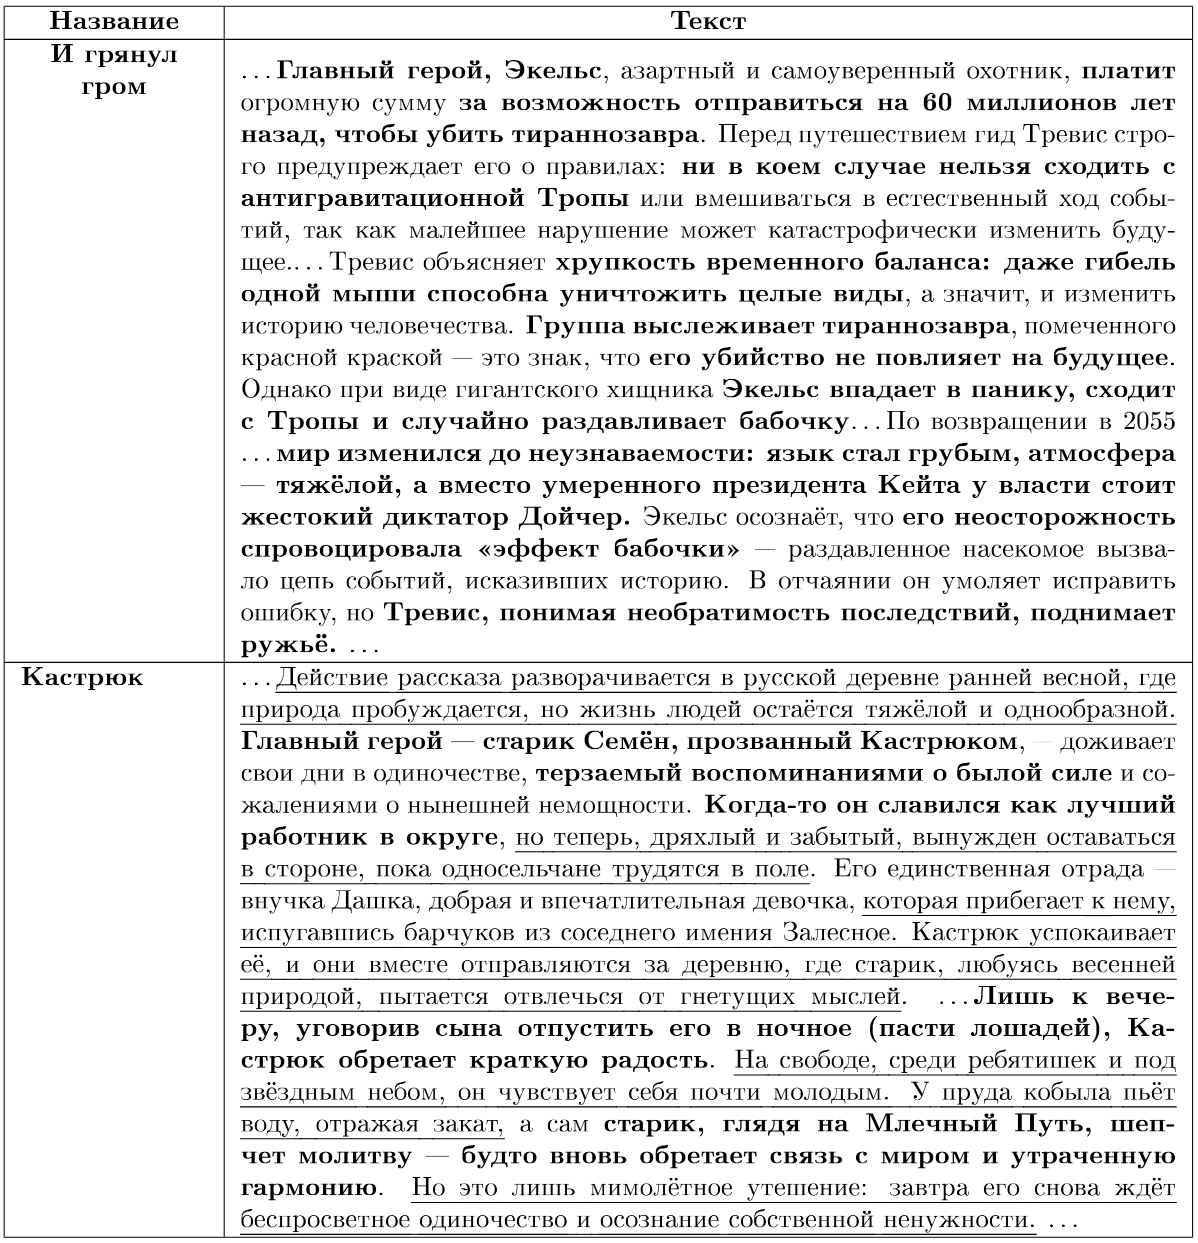
\includegraphics[width=0.9\textwidth]{figures/two_ref.png}
  \caption{Comparison of the best and worst generated synopses}
  \label{fig:refs}
\end{figure}

\begin{figure}[ht!]
  \centering
  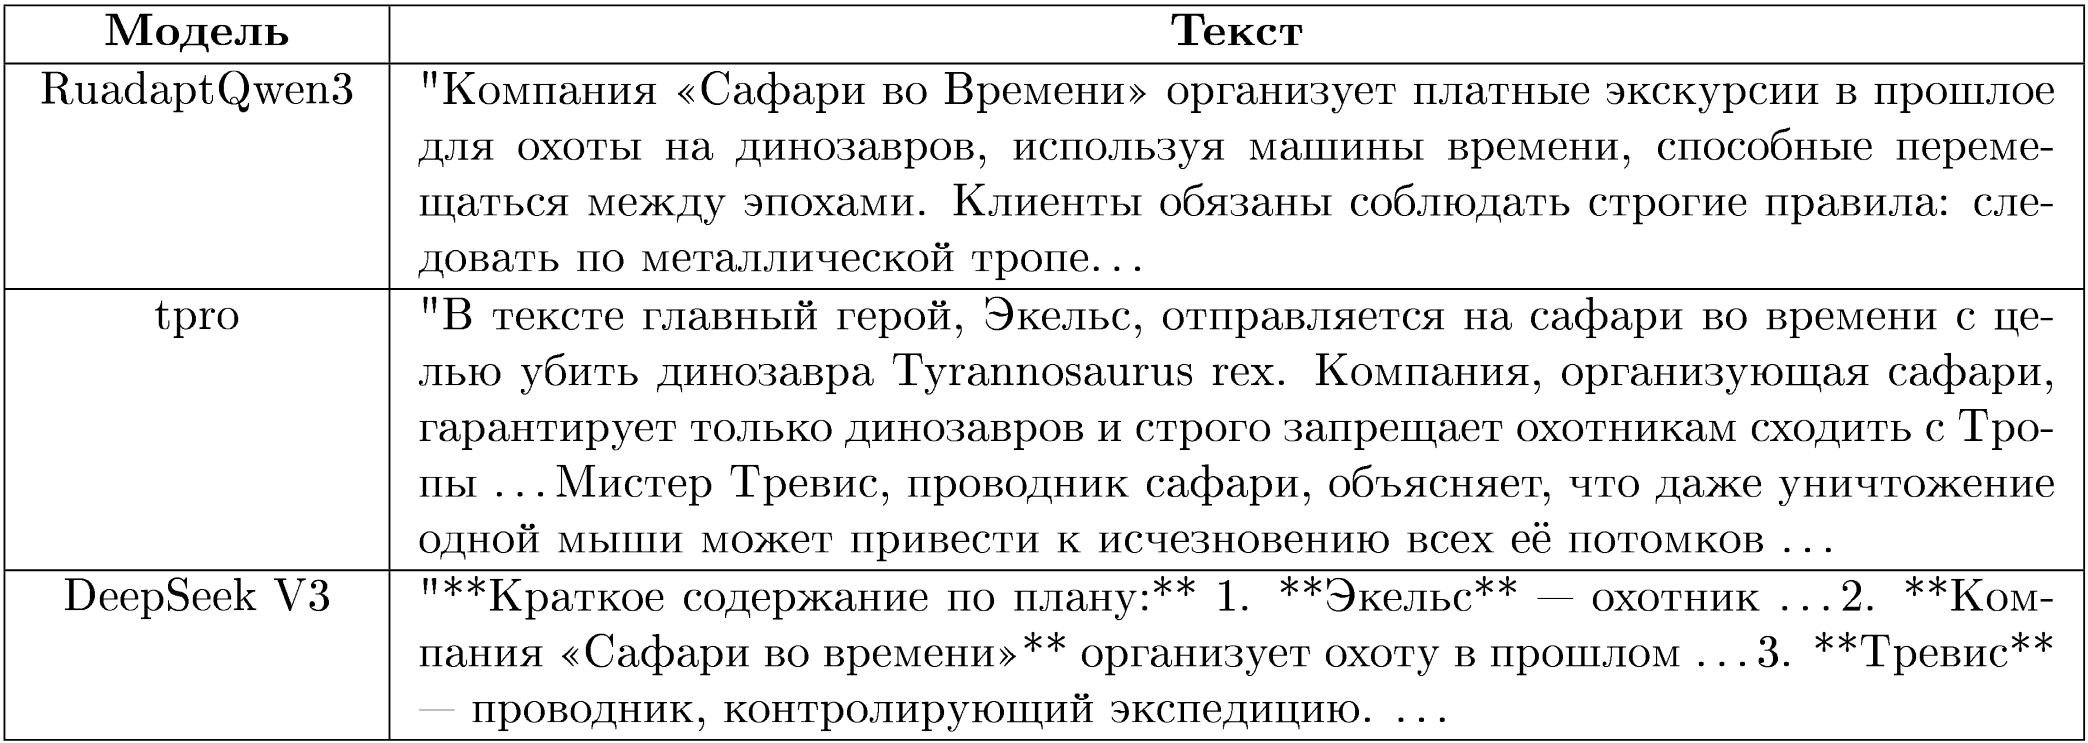
\includegraphics[width=0.9\textwidth]{figures/three_ref.png}
  \caption{Model comparison for blueprint-based synopses}
  \label{fig:bl_ref}
\end{figure}

Comparing models, DeepSeek V3 generally outperforms smaller models; however, within the blueprint method, in 30\% of cases
RuadaptQwen3-32B-Instruct-v2 performs best, and tpro in 43\%. For reference, consider the synopsis for "A Sound of Thunder" generated with the blueprint method,
with small excerpts shown in Figure \ref{fig:bl_ref}.
While the DeepSeek V3 synopsis resembles a numbered list of main events,
the outputs from RuadaptQwen3-32B-Instruct-v2 and tpro are cohesive narratives that cover the key plot points.

Note that the best result overall was achieved by the blueprint method with the large model Qwen3-235B-A22B,
as shown in Table \tabref{tab:results_models}. For comparison, on the story "Barbos and Zhulka",
the hierarchical method with Qwen3-235B-A22B misclassified "Zhulka" as a horse rather than a dog. Also, DeepSeek V3 tends to strictly follow the blueprint template and produces a numbered list
of key events and main characters, rather than a flowing synopsis, whereas Qwen3-235B-A22B writes plain text.
Thus, the unmodified blueprint method delivered the best results when using the strongest available model - Qwen3-235B-A22B.

\subsection{Time measurements.}
The results in seconds (average of three runs) are in Table \tabref{tab:timing}.
They confirm that modifications speed up generation.

\tab{tab:timing}{Generation time (seconds) for a text of 81{,}049 characters (11 chunks).}{
  \small
\begin{tabular}{lcccc}
\textbf{Model} & \makecell{Hierarchical} & \makecell{Hierarchical\\with filtering} & \makecell{Blueprint} & \makecell{Blueprint\\with clustering} \\
\hline
DeepSeek V3                  & 237.83 & 72.42 & 292.80 & 268.75 \\
Qwen3-235B-A22B              & 113.24 & 39.45 & 215.63 & 145.20 \\
\hline
RuadaptQwen3-32BInstruct-v2  & 218.23 & 72.54 & 420.95 & 470.4 \\
tpro                         & 472.23 & 127.38 & 421.65 & 185.94 \\
\hline
RuadaptQwen2.5-7B-Lite-Beta  & 84.64 & 25.70 & 103.66 & 78.99 \\
yagpt5lite                   & 34.17 & 14.08 & 99.70 & 27.26 \\
\end{tabular}
}

Interestingly, ultra-large models such as Qwen3-235B-A22B and DeepSeek V3 showed higher speed
than some 32B models.
A key reason is the Mixture-of-Experts (MoE) architecture:
during generation only a subset of parameters is active (e.g., ~30B out of ~600B),
and such models are typically optimized further for throughput.

% ================= ЗАКЛЮЧЕНИЕ =================

\section*{Conclusion}
We presented the first open dataset that pairs book texts with their synopses from the “Narodny Briefly” resource \cite{Briefly}.
We proposed two improved LLM-based approaches to summarizing fiction: hierarchical with filtering and blueprint with clustering.
The hierarchical method with filtering speeds up generation with minimal quality loss,
making it suitable for long works under limited model context.

Our comparative analysis shows that large models such as DeepSeek V3 and Qwen3-235B-A22B generally deliver higher QA coverage and
more complete synopses than compact models, especially with hierarchical and blueprint methods.
However, for certain text types and methods (e.g., baseline blueprint), more compact models such as RuadaptQwen3-32B-Instruct-v2
can be competitive at lower compute cost.
Thus, model choice should balance available resources, quality requirements, and the nature of the processed texts.

\section*{Acknowledgements}
The study was supported by grant No. 25-11-00191 from the Russian Science Foundation.
The work was carried out using the supercomputer "MSU-270" of the Lomonosov Moscow State University.
% ================= ЛИТЕРАТУРА =================



\openaccess

\bibliographystyle{superfri}
\begin{thebibliography}{99}
\bibitem{BookSum}
BOOKSUM: A Collection of Datasets for Long-form Narrative Summarization / Wojciech Kryscinski, Nazneen Rajani, Divyansh Agarwal et al. // Findings of the Association for Computational Linguistics: EMNLP 2022 / Ed. by Yoav Goldberg, Zornitsa Kozareva, Yue Zhang. - Abu Dhabi, United Arab Emirates: Association for Computational Linguistics, 2022. - . - Pp. 6536-6558. https://aclanthology.org/2022.findings-emnlp.488/.

\bibitem{alexandria}
Echoes from Alexandria: A Large Resource for Multilingual Book Summarization / Alessandro Scir`e, Simone Conia, Simone Ciciliano, Roberto Navigli // Findings of the Association for Computational Linguistics: ACL 2023 / Ed. by Anna Rogers, Jordan Boyd-Graber, Naoaki Okazaki. - Toronto, Canada: Association for Computational Linguistics, 2023. - . - Pp. 853-867. https://aclanthology.org/2023.findings-acl.54/.

\bibitem{fables}
FABLES: Evaluating faithfulness and content selection in book-length summarization \\/ Yekyung Kim, Yapei Chang, Marzena Karpinska et al. // First Conference on Language Modeling. - 2024. https://openreview.net/forum?id=YfHxQSoaWU.

\bibitem{Briefly}
\textit{Народный Брифли.}  
Электронная библиотека кратких пересказов литературных произведений.  
\url{https://wiki.briefly.ru/} (дата обращения: 30.07.2025).

\bibitem{librusec}
Библиотека художественных произведений.  
\url{https://librusec.org//} (дата обращения: 30.07.2025).

\bibitem{hierarchical} 
Wu J. et al. Recursively Summarizing Books with Human Feedback //arXiv e-prints. - 2021. - С. arXiv: 2109.10862.

\bibitem{blueprint} 
Text-Blueprint: An Interactive Platform for Plan-based Conditional Generation / \\Fantine Huot, Joshua Maynez, Shashi Narayan et al. // Proceedings of the 17th Conference of the European Chapter of the Association for Computational Linguistics:
System Demonstrations / Ed. by Danilo Croce, Luca Soldaini. - Dubrovnik, Croatia: Association for Computational Linguistics, 2023. - . - Pp. 105-116. https:
//aclanthology.org/2023.eacl-demo.13/.

\bibitem{rouge}
\textit{ROUGE.}
Lin C. Y. Rouge: A package for automatic evaluation of summaries //Text summarization branches out. - 2004. - С. 74-81.

\bibitem{bertscore}
\textit{BERTScore.}
BUCKLEY C. Evaluating Evaluation Measure Stability //ACM SIGIR 2000 Proceedings. - 2000.

\bibitem{qwen3}
\textit{Qwen3-235B.}
Yang A. et al. Qwen3 technical report //arXiv preprint arXiv:2505.09388. - 2025.

\bibitem{ruadapt}
\textit{RuadaptQwen.}
Tikhomirov M., Chernyshev D. Facilitating large language model russian adaptation with learned embedding propagation //Journal of Language and Education. - 2024. - Т. 10. - №. 4 (40). - С. 130-145.

\bibitem{deepseek}
\textit{DeepSeek V3.}
Liu A. et al. DeepSeek-V3 Technical Report //CoRR. - 2024.

\bibitem{tpro}
Т-Банк открыл доступ к собственной русскоязычной языковой модели в весовой категории 7-8 млрд параметров\\ Т-Банк URL: https://www.tbank.ru/about/news/20072024-t-bank-opened-access-its-own-russian-\\language-language-model-weight-category-of-7-8-billion-parameters/ (дата обращения: 10.05.2025).

\bibitem{yagpt}
YandexGPT 5 с режимом рассуждений // Яндекс URL: https://ya.ru/ai/gpt?ysclid=mal9jrssc8906806775 (дата обращения: 30.07.2025).

\end{thebibliography}

\end{document}
